% *** Acids and Bases ***
\chapter{Acids and Bases}
\section{Pre-lesson exercise: Acids and Bases}
\subsection{Acid--base reactions}
\subsubsection{Problem}
Which of the following are \hil{acid--base reactions}
according to the Brønsted--Lowry theory? For the acid--base
reactions in this set, identify the \hil{conjugate acid}
(with its corresponding base\sidenote{A proton-donating substance})
and the \hil[cobalt]{conjugate base} (with its corresponding acid\sidenote{A proton-accepting substance}).

\begin{itemize}
	\item \ch{H2SO4 + H2O -> HSO4- + H3O+}
	\item \ch{(CH3)3N + H2O -> (CH3)3NH^{+} + OH-}
	\item \ch{2 Na + H2O -> 2 NaOH + H2}
	\item \ch{HCl + HCO3- -> Cl- + H2CO3}
	\item \ch{Cl2 + H2 -> 2 HCl}
	\item \ch{CH4 + Cl2 -> CH3Cl + HCl}
\end{itemize}

\subsubsection{Solution}
\begin{itemize}
	\item {\color{accent} \ch{H2SO4 + H2O -> HSO4- + H3O+}}
	      \begin{itemize}
		      \item The acid is \ch{H2SO4}, and its conjugate base is \ch{HSO4-}.
		      \item The base is \ch{H2O}, and its conjugate acid is \ch{H3O+}.
	      \end{itemize}
	\item {\color{accent} \ch{(CH3)3N + H2O -> (CH3)3NH^{+} + OH-}}
	      \begin{itemize}
		      \item The acid is \ch{H2O}, and its conjugate base is \ch{OH-}.
		      \item The base is \ch{(CH3)3N}, and its conjugate acid is \ch{(CH3)3NH^{+}}.
	      \end{itemize}
	\item \ch{2 Na + H2O -> 2 NaOH + H2} is \textbf{not} an acid--base reaction.
	\item {\color{accent} \ch{HCl + HCO3- -> Cl- + H2CO3}}
	      \begin{itemize}
		      \item The acid is \ch{HCl}, and its conjugate base is \ch{Cl-}.
		      \item The base is \ch{HCO3-}, and its conjugate acid is \ch{H2CO3}.
	      \end{itemize}
	\item \ch{Cl2 + H2 -> 2 HCl} is \textbf{not} an acid--base reaction.
	\item {\color{black!40!white} \ch{CH4 + Cl2 -> CH3Cl + HCl}} is a \hil[naples]{disproportionation reaction}.
\end{itemize}

\subsection{Conjugate acids and bases}

\subsubsection{Problem}
Which of the following are
\hil[naples]{conjugate acid--base pairs}\sidenote{Two species that differ by one proton}?

\begin{enumerate}
	\item \ch{CH3CO2H} and \ch{CH3CO2-}
	\item \ch{HCO3-} and \ch{CO3^2-}
	\item \ch{SO3} and \ch{HSO3-}
	\item \ch{[Al(H2O)6]^3+} and \ch{[Al(H2O)5(OH)]^2+}
	\item \ch{BH3} and \ch{BH4-}
	\item \ch{H-} and \ch{H2}
\end{enumerate}
\subsubsection{Solution}
\begin{itemize}
	\item {\color{accent} \ch{CH3CO2H} and \ch{CH3CO2-}} are a conjugate acid--base pair.
	\item {\color{accent} \ch{HCO3-} and \ch{CO3^2-}} are a conjugate acid--base pair.
	\item \ch{SO3} and \ch{HSO3-} are \textbf{not} a conjugate acid--base pair.
	\item {\color{accent} \ch{[Al(H2O)6]^3+} and \ch{[Al(H2O)5(OH)]^2+}} are a conjugate acid--base pair.
	\item \ch{BH3} and \ch{BH4-} are \textbf{not} a conjugate acid--base pair.
	\item {\color{accent} \ch{H-} and \ch{H2}} are a conjugate acid--base pair.
\end{itemize}

% *** homework ***
\pagebreak
\section{Homework: Acids and Bases}
\subsection{Polyprotic acids}
\subsubsection{Problem}
In a \hil{polyprotic acid} \sidenote{A substance capable of donating more than one proton},
we have successive \(\Ka\) values for each successive
dissociation. For example, phosphoric acid has three dissociations, and so has
correspondingly three \(\Ka\) values, one for each dissociation (Equations~\ref{eq:polyprotic}):
\begin{align*}
	\ch{H3PO4 \aq{}     & <=> H^{+} \aq{} + H2PO4- \aq}    \nonumber                      \\
	\ch{H2PO4- \aq{}    & <=> H^{+} \aq{} + HPO4^{2-} \aq} \nonumber                      \\
	\ch{HPO4^{2-} \aq{} & <=> H^{+} \aq{} + PO4^{3-} \aq} \nonumber \label{eq:polyprotic}
\end{align*}

The corresponding \Ka\ values are
\begin{align*}
	K_1 & = \num{7.11e-3}  \\
	K_2 & = \num{6.32e-8}  \\
	K_3 & = \num{4.48e-13}
\end{align*}

\begin{enumerate}
	\item\label{item:decreased-ka} Suggest why, for most polyprotic acids, the successive \(\Ka\) values
	      will decrease by a large factor.
	\item\label{item:significance} \bf{Assuming only the first dissociation of phosphoric acid is significant},
	      calculate the \pH\ of \qty{0.0750}{\conc} phosphoric acid.
	\item Based on your answer to Part~\ref{item:decreased-ka}, estimate \ch{[H3PO4]},
	      \ch{[H2PO4^{-}]}, \ch{[HPO4^{2-}]} and \ch{[PO4^{3-}]} in the phosphoric acid
	      solution. From your calculations, is the assumption in Part~\ref{item:significance}
	      valid?
\end{enumerate}

\subsubsection{Solution}
It becomes more difficult for polyprotic acids to lose \ch{H+} ions with each
dissociation, since {\color{accent} \ch{H+} ions are less likely to leave an increasingly
		negatively-charged anion}.
\begin{equation*}
	K_1 = \frac{\ch{[H^{+}]} \ch{[H2PO4^{-}]}}{\ch{[H3PO4]}}
\end{equation*}
We can construct an ICE table, where \(x\) is the change in concentration of
each species (Table~\ref{tab:h3po4}).
\begin{table}[htpb]
	\centering
	\begin{tabular}{l r r r}
		\toprule
		\textbf{Concentration / \unit{\conc}} & \ch{H3PO4}           & \ch{H+} & \ch{H2PO4^{-}} \\
		\midrule
		Initial                               & \num{0.0750}         & 0       & 0              \\
		Change                                & \(-x\)               & \(+x\)  & \(+x\)         \\
		End                                   & \(\num{0.0750} - x\) & \(x\)   & \(x\)          \\
		\bottomrule
	\end{tabular}
	\caption{ICE table for the dissociation of \ch{H3PO4}}
	\label{tab:h3po4}
\end{table}

Hence, by assuming that only the dissociation of \ch{H3PO4} is significant,
\begin{align*}
	\num{7.11e-3} & = \f{x^2}{\num{0.0750} - x}  \\
	x             & = \qty{1.981e-2}{\conc}      \\
	\pH           & = -\lg x                     \\
	              & = \color{accent} \num{1.703}
\end{align*}

Hence,
\begin{align*}
	\ch{[H3PO4]}   & \approx 0.0750 - x     \\
	               & = \qty{0.05519}{\conc} \\
	\ch{[H2PO4^-]} & \approx x              \\
	               & = \qty{0.01981}{\conc}
\end{align*}

Let \(y\) be \ch{[HPO4^{2-}]} formed by the second dissociation.
\begin{align*}
	K_2 & = \f{\ch{[H^+]} \ch{[HPO4^{2-}]}}{\ch{[H2PO4^-]} - y} \\
	    & = \f{y \ab(y + \num{0.01981})}{\num{0.01981} - y}     \\
	y   & = \qty{6.3e-8}{\conc}
\end{align*}

Since \(y\) is minuscule compared to \(x\), the assumption in
Part~\ref{item:significance} can be accepted.

Let \(z\) be \ch{[PO4^{3-}]} formed by the third dissociation.
\begin{align*}
	K_3 & = \f{\ch{[H^+]} \ch{[PO4^{3-}]}}{\ch{[H2PO4^-]} - z} \\
	    & = \f{z \ab(z + \num{0.01981})}{y-z}                  \\
	z   & \approx 0
\end{align*}
Since \(z \approx 0\), the assumption in
Part~\ref{item:significance} can be accepted for the third dissociation also.

\subsection{Titration curves}
\subsubsection{Problem}
Sketch the titration curve of \ch{H2SO3}, a diprotic weak acid, against
\ch{NaOH} \sidenote{\ch{NaOH} is a strong base.}.
Suggest the indicators you would add in order to see both end points clearly, and
state their colour changes.

\subsubsection{Solution}
\ch{H2SO3} dissociates according to the following equations:
\begin{align*}
	\ch{H2SO3 \aq{}  & <=> HSO3^- \aq{} + H^+ \aq}   \\
	\ch{HSO3^- \aq{} & <=> SO3^{2-} \aq{} + H^+ \aq}
\end{align*}
Since \ch{H2SO3} is a weak acid, the increase in \pH\ will be more gradual
than those expected with a strong acid.
\begin{figure}[htpb]
	\centering
	\begin{tikzpicture}
		\begin{axis}[ticks=none, xlabel={Volume of \ch{NaOH} added}, ylabel={pH}]
			% Adding points manually based on assumed calculations
			\addplot[
				smooth,
			] coordinates {
					% step 1
					(0, 1.9) (5, 1.93) (10, 1.95) (15, 1.975)
					(20, 2) (22, 2.1) (24, 2.25) (26, 2.35)
					(28, 2.4) (30, 2.5) (32, 2.7) (34, 2.9)
					(36, 3.2) (38, 3.5) (39, 3.75) (40, 4)
					% step 2
					(42, 4.5) (44, 5) (46, 5.5) (48, 6) (50, 6.2)
					(52, 6.4) (54, 6.6) (56, 6.8) (58, 6.9) (59, 6.95)
					(60, 7) (61, 7.05) (62, 7.07) (63, 7.1) (65, 7.15)
					(67, 7.2) (68, 7.22) (70, 7.24) (72, 7.51) (74, 7.82)
					(76, 8.44) (78, 8.87) (79, 9.5) (80, 10) (82.5, 10.5)
					(85, 11) (87.5, 11.5) (89, 12) (90, 12) (95, 12) (97, 12)
					(100, 12) (105, 12) (110, 12) (115, 12) (118, 12) (120, 12)
				};
			\addplot+ [only marks] coordinates {
					(40, 4) (80, 10)
				};
		\end{axis}
	\end{tikzpicture}
	\caption{Titration curve of \ch{H2SO3} with \ch{NaOH}}
	\label{fig:titration-h2so3}
\end{figure}

The titration curve is in Figure~\ref{fig:titration-h2so3}. We can use {\color{accent}
		methyl orange} for the first endpoint, and {\color{accent} phenolphthalein} for the second.

\subsection{Liquid--liquid extraction}
\subsubsection{Problem}
Liquid--liquid extraction (Figure~\ref{fig:ll-sep}) is a technique to separate
organic compounds using a separatory funnel. The crude sample is first dissolved
in an organic solvent such as hexane and this solution is poured into a separatory funnel.
Next, water is added to the separatory funnel and the funnel is shaken.
Because hexane and water are immiscible, they form two layers in the
separatory funnel. The organic compound that is more soluble in water will migrate
from the hexane layer to the water layer. The two layers contain different
compounds and can be collected separately.

\begin{wrapfigure}{r}{0.5\textwidth}
	\centering
	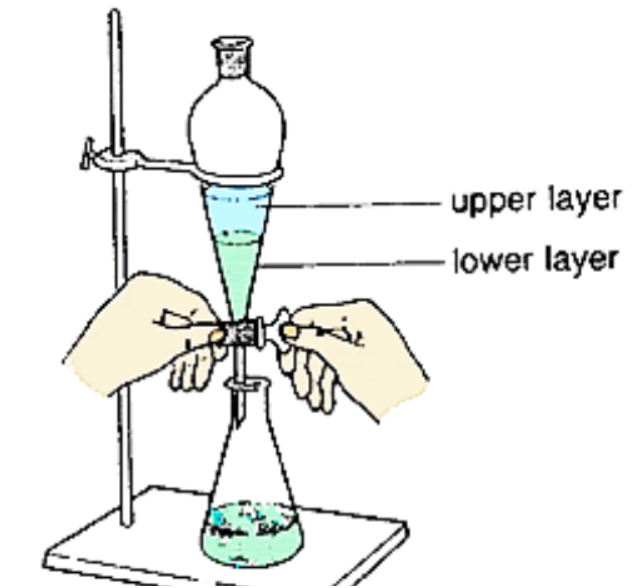
\includegraphics[width=0.5\linewidth]{assets/08_ll_separation.png}
	\caption{Liquid--liquid separation}
	\label{fig:ll-sep}
\end{wrapfigure}

You are given a sample containing both phenol (\(\pKa = \num{9.95}\)) and benzoic
acid (\(\pKa = \num{4.20}\)). Both compounds are not very soluble in water. To
improve the separation, aqueous sodium bicarbonate (\ch{NaHCO3}) can be used instead
of water.

It is given that \(\pKa_1 = \num{6.3}\) and \(\pKa_2 = \num{10.3}\) for carbonic
acid, \ch{H2CO3}. In which layer will the majority of the benzoic acid be found?
In which layer will the majority of the phenol be found? You need not perform
equilibrium computations.

\subsubsection{Solution}
\ch{NaHCO3} is a weak base. We can write
\begin{equation*}
	\ch{HCO3^- \aq{} <=> CO3^{2-} \aq{} + H^+ \aq}
\end{equation*}
We can also write the dissociation of \ch{H2CO3 \aq} as
\begin{align*}
	\ch{H2CO3 \aq{}    & <=> HCO3^{-} \aq{} + H^+ \aq} \\
	\ch{HCO3^{-} \aq{} & <=> CO3^{2-} \aq{} + H^+ \aq}
\end{align*}
It is the \it{second} dissociation of \ch{H2CO3 \aq} we desire. We use
\(\pKa \coloneqq \pKa_2 = \num{10.3}\).

Since the \pKa\ of benzoic acid (\num{4.20}) is smaller than that of phenol
(\num{9.95}), it has a larger \Ka\ and hence is the stronger acid. It will react
more readily with the \ch{NaHCO3 \aq} to form benzoate ions, which are soluble
in water. {\color{accent} The majority of the benzoic acid will be found in the
		aqueous layer.}

On the other hand, the \pKa\ values of phenol and \ch{H2CO3 \aq} are closer
to each other, making the acid--base reaction less favourable. {\color{accent}
		Phenol will predominantly be found in the hexane layer.}

